\section{Objects for distributed systems}

The effective distribution of Logical Nodes 
on diferents IEDs  
is a reality thanks to researches about 
the structure of distributed systems. More 
than 20 years ago emerged requirements 
for the object paradigm to suport the 
design and development of distributed systems.

Theses quotes were extracted from Jazayeri 
1988 research:

\emph{
``An object on one node can send a (multicast) message 
to several other objects \ldots''
} (MCAA) \todo{completar y ver si esta bien}

\emph{
`` \ldots The ability to group 
a set of objects and address them as one entity 
is important in many applications both from an 
efficiency point of view and from a program 
structuring point of view \ldots'' 
} (DO, DATA-SET, FCD, FCDA)\todo{completar y ver si esta bien}

\emph{
`` \ldots a final 
difference is that our objects are active and 
not reactive, in the sense that they can start 
up spontaneosly performing operations, not 
necessarily only in response to method invocations.
Such a facility is useful, for example, to allow objects 
to monitor the enviroment and change their behavior based 
on changes in the enviroment \ldots'' 
} (Some active objects 
are GOOSE, URCB and some passive object 
are \todo{completar y ver si esta bien})

\cite{Jazayeri:1988}.



\begin{figure}
  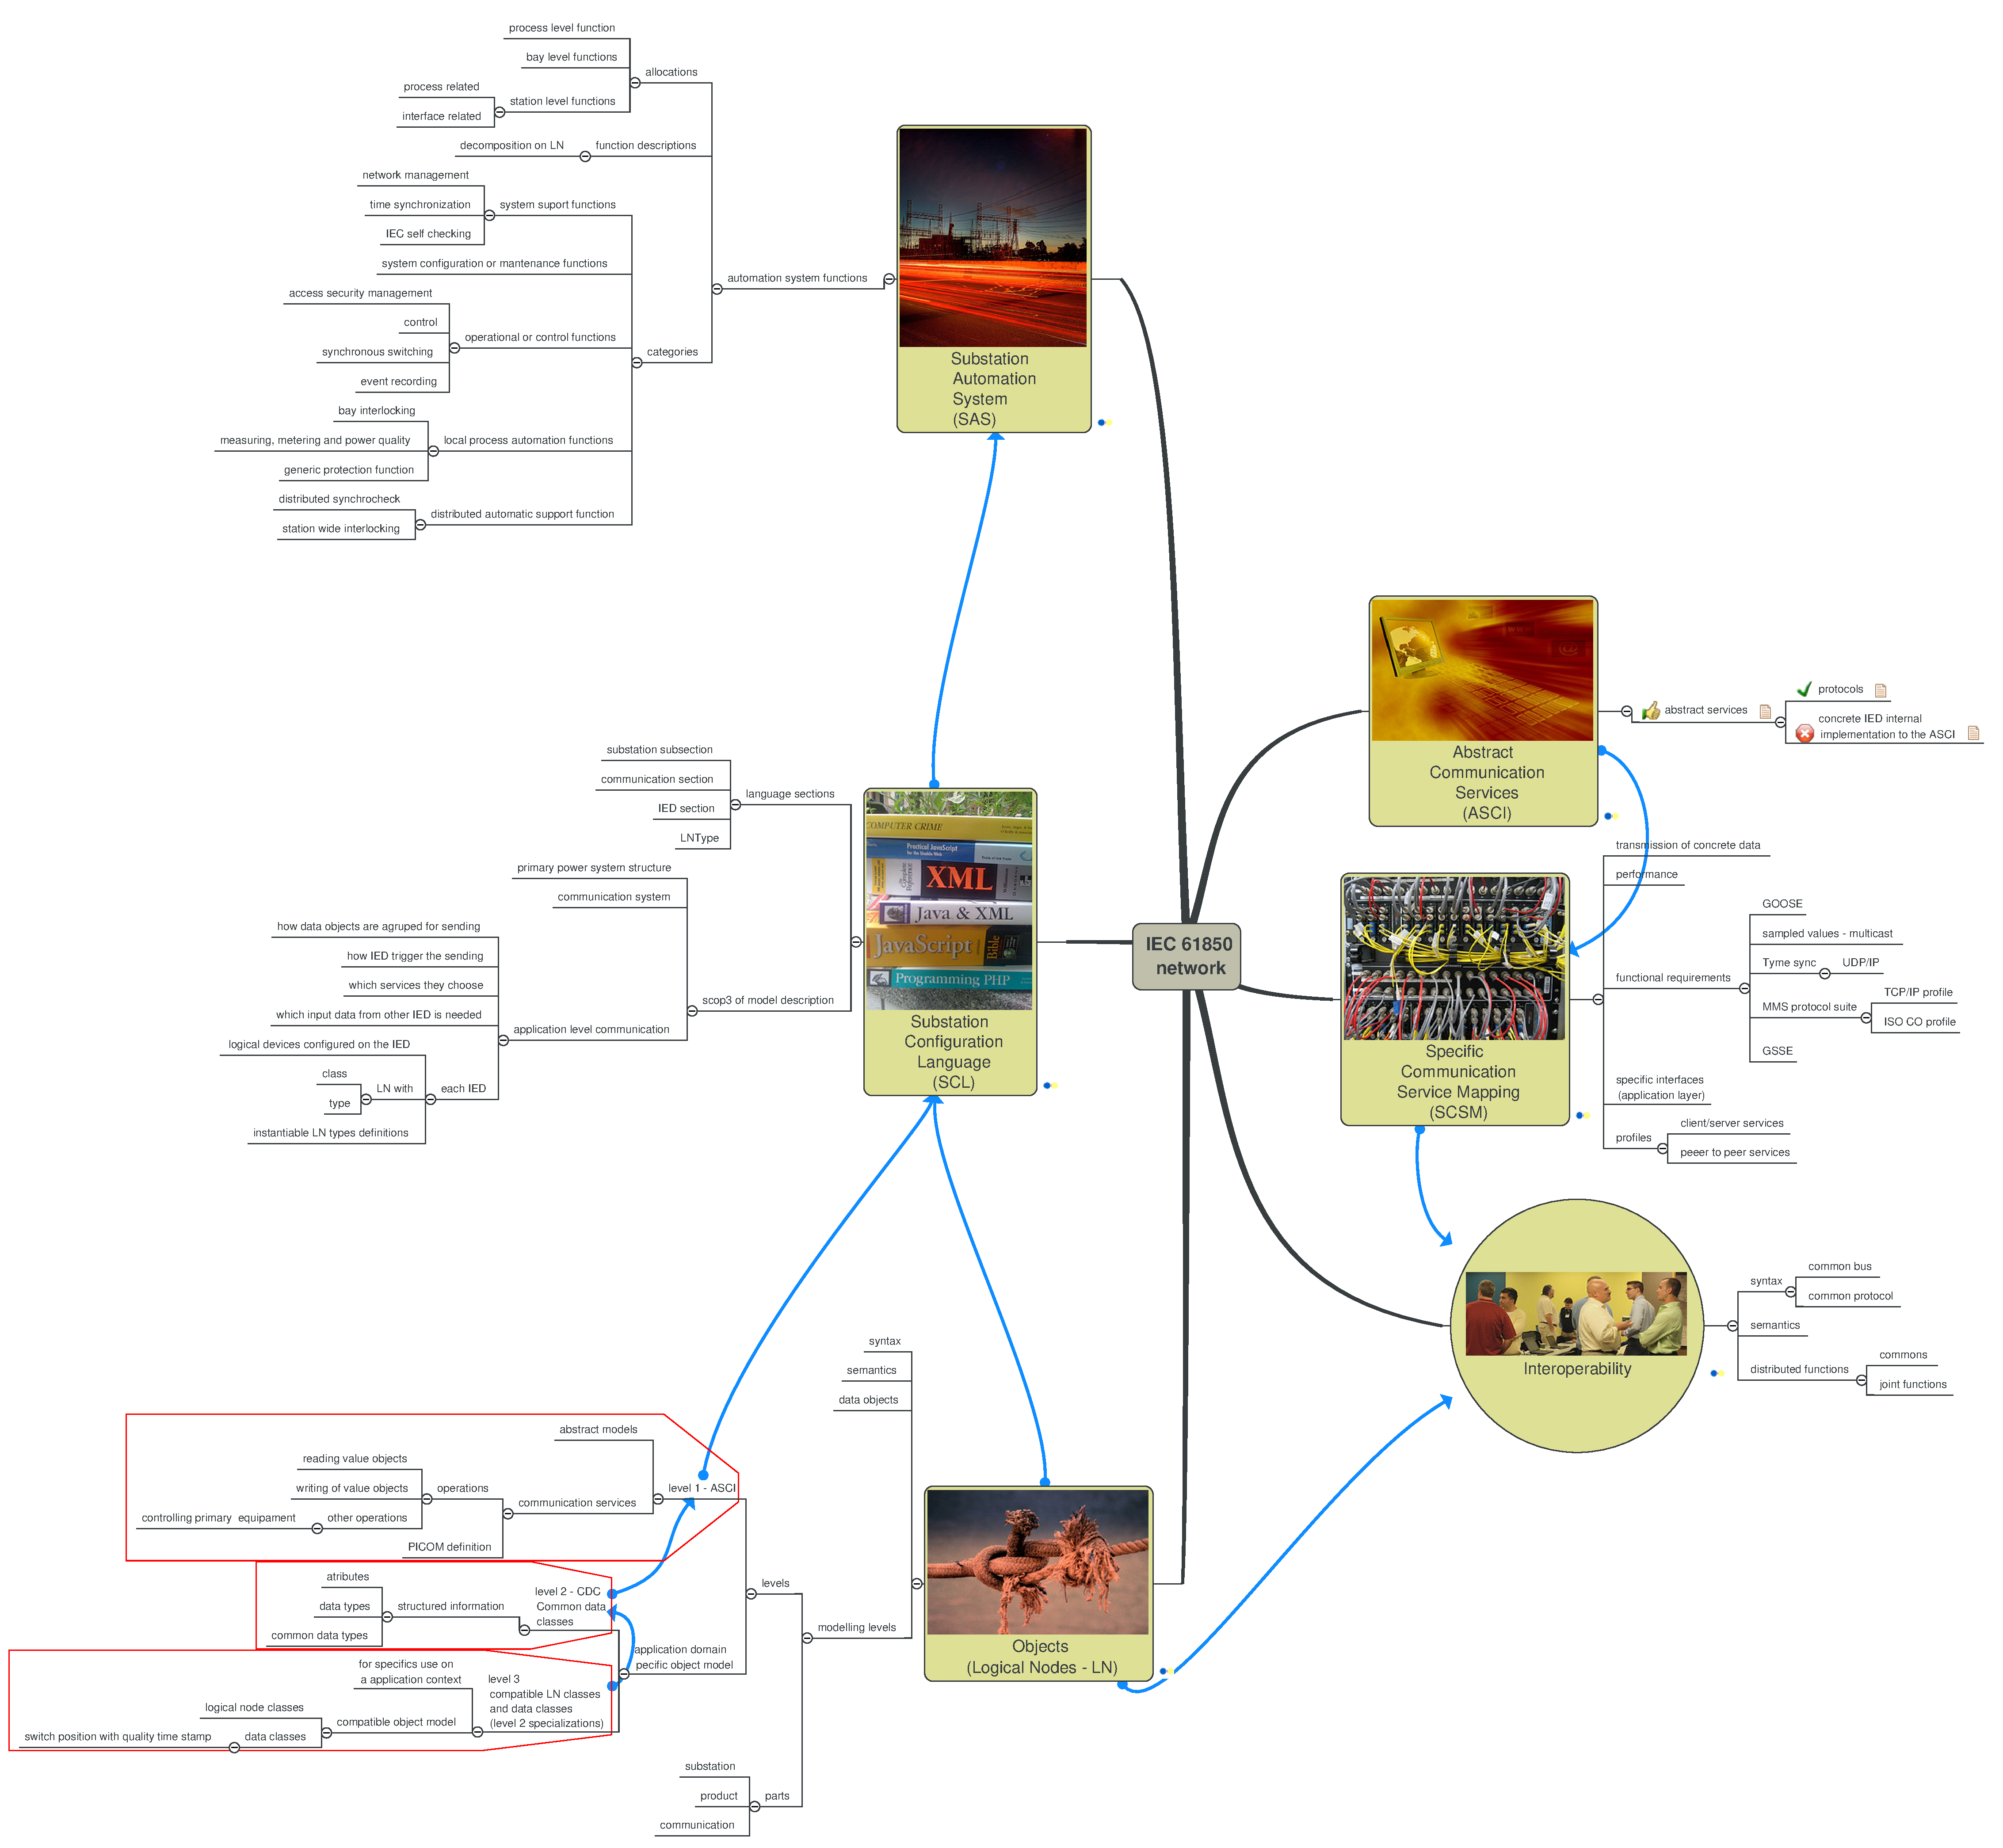
\includegraphics[width=1.0\textwidth]{appendices/IEC61850network}
  \caption{Borrador - Parte del esquema del futuro capitulo }
  \label{fig:lan-networks-topologies-fig1}
\end{figure}


\begin{figure}
  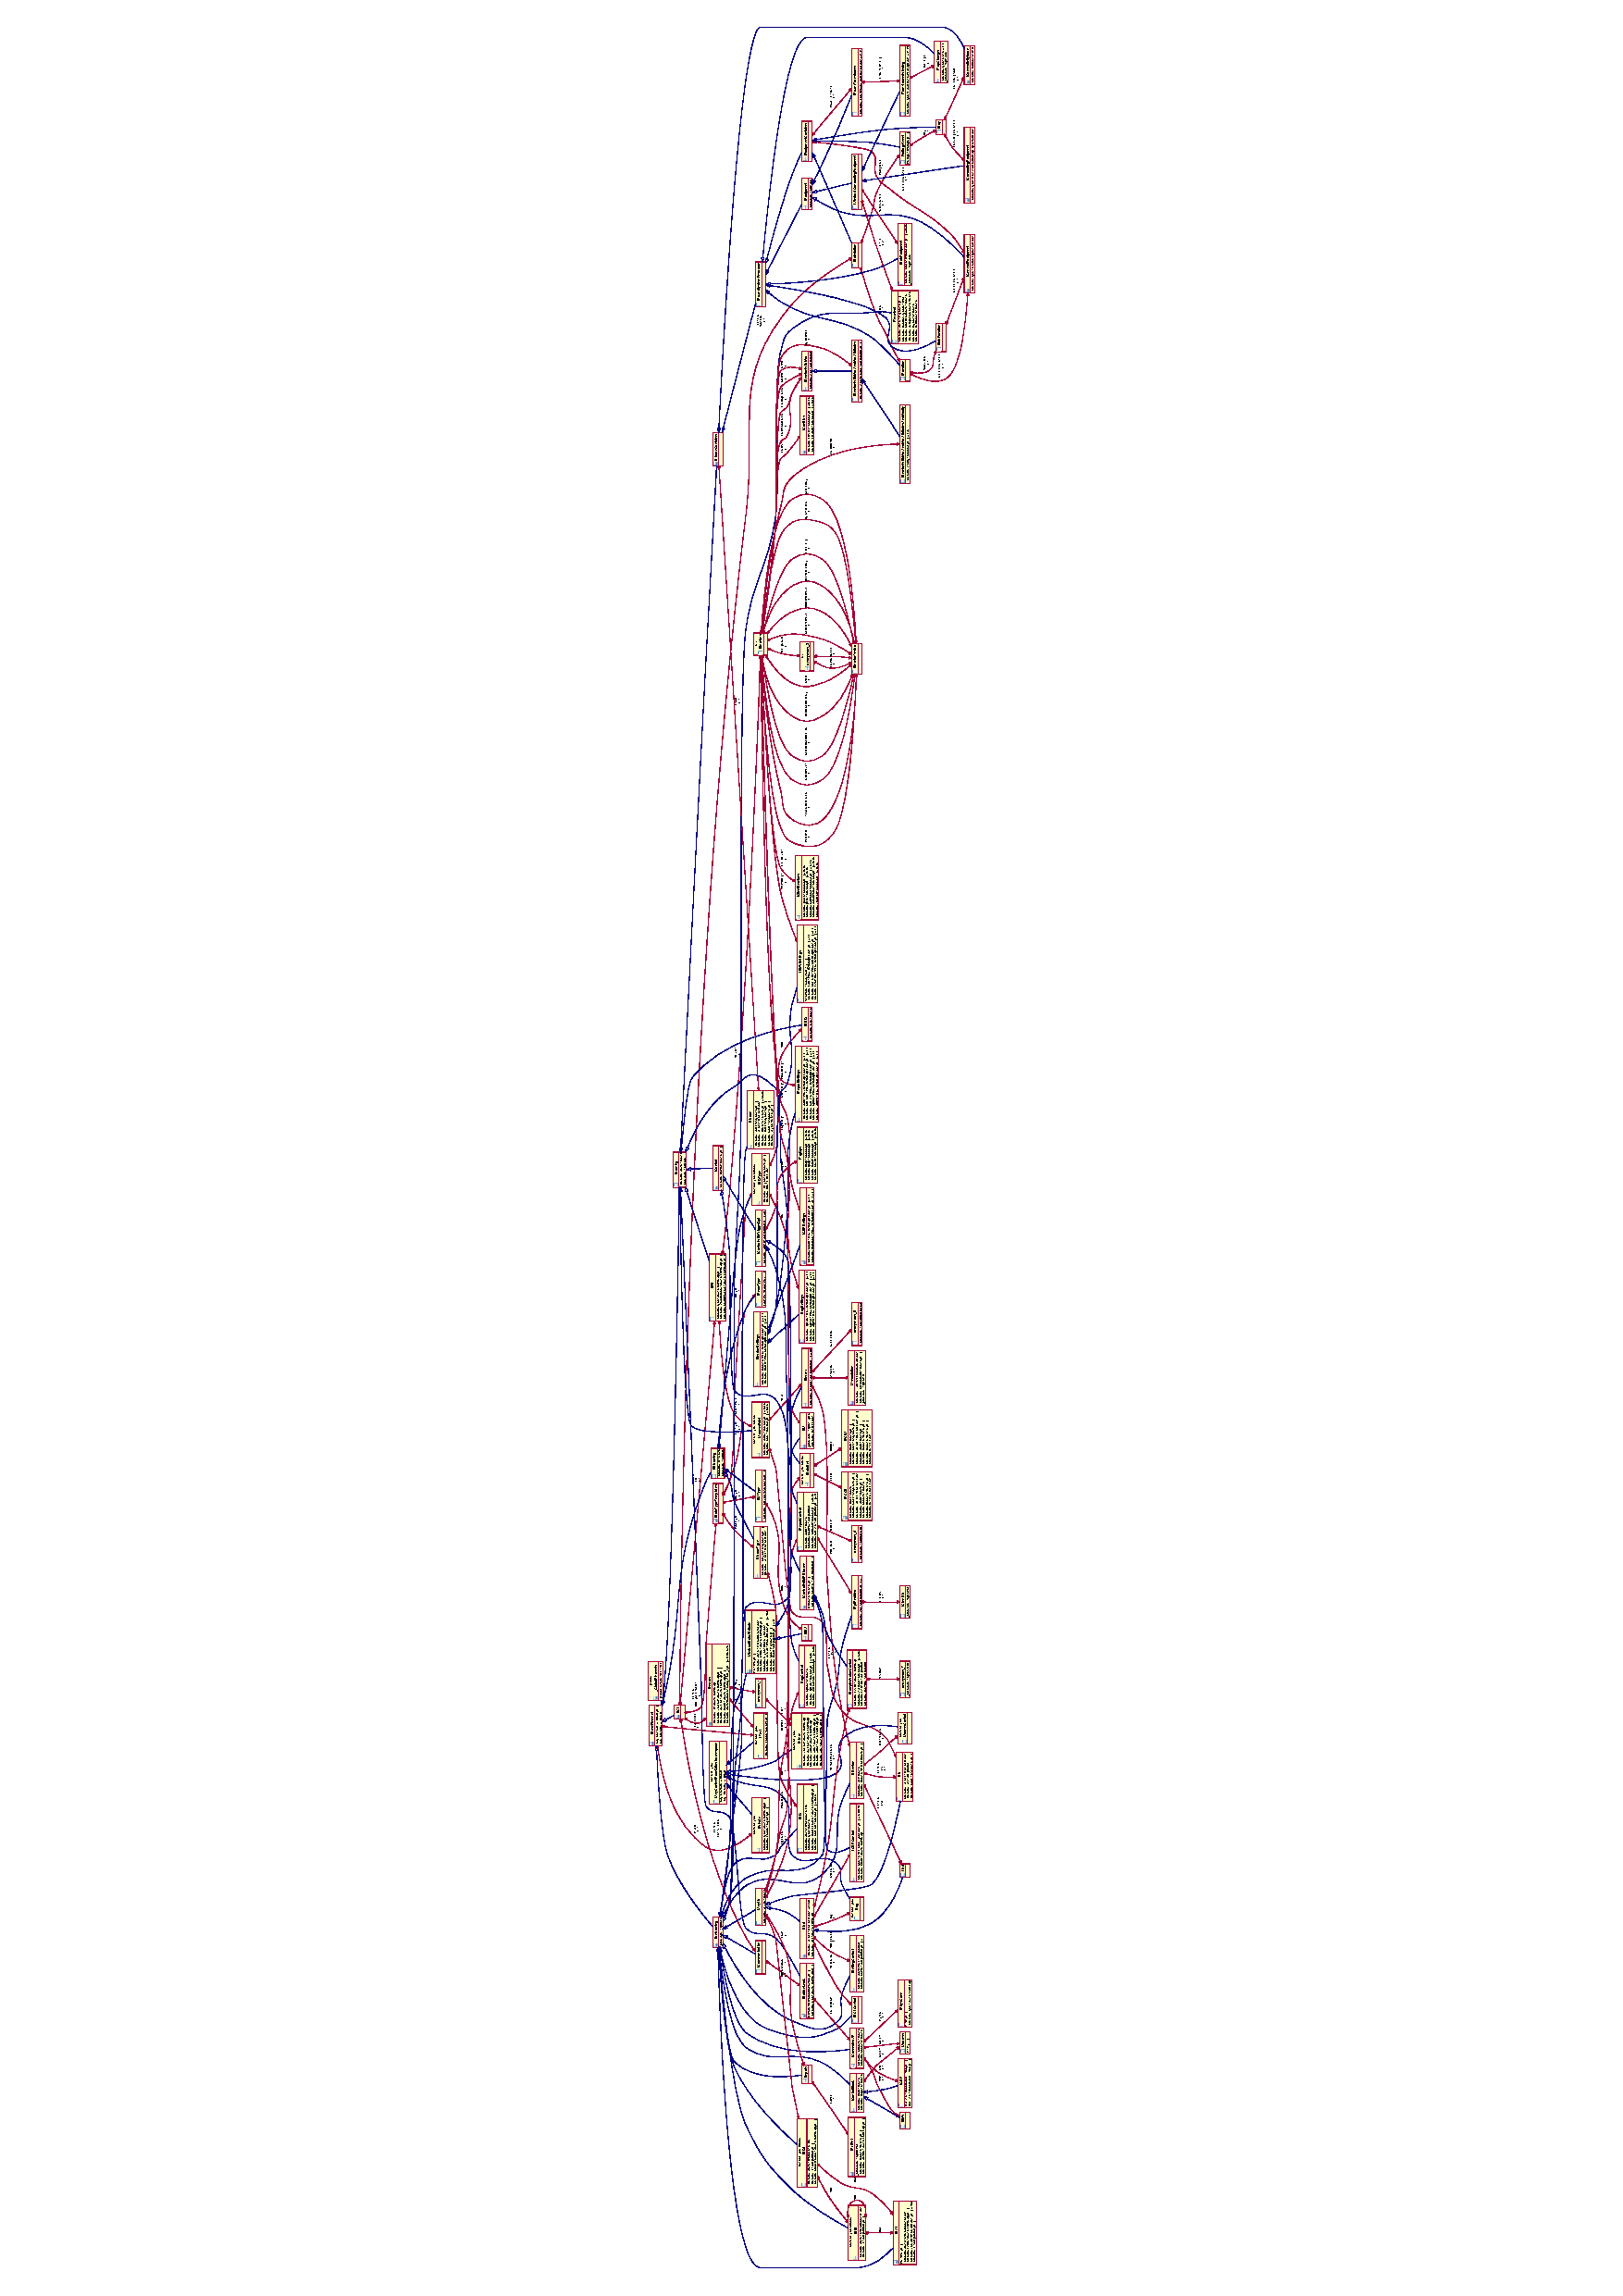
\includegraphics[width=1.0\textwidth]{appendices/JavaPrinting}
  \caption{Borrador - Parte del esquema del futuro capitulo }
  \label{fig:lan-networks-topologies-fig2}
\end{figure}
 
